
\chapter{NAO Kinematics: The Problem}
\label{problem}

\section{NAO Robot Specifications}
Aldebaran NAO is a humanoid robot with five kinematic chains (head, two arms, two legs). It is 58cm tall and it has about 5kg of mass. The version we are working on is the RoboCup edition v3.3 with 21 DOF. NAO has two DOF on the head, four DOF on each arm, five DOF on each leg, and one DOF in the pelvis, which is shared between the two legs. The five kinematic chains and their joints are the following:
\begin{description}
\item[Head:] HeadYaw, HeadPitch
\item[Left Arm:] LShoulderPitch, LShoulderRoll, LElbowYaw, LElbowRoll
\item[Right Arm:] RShoulderPitch, RShoulderRoll, RElbowYaw, RElbowRoll
\item[Left Leg:] LHipYawPitch, LHipRoll, LHipPitch, LKneePitch, LAnklePitch, LAnkleRoll
\item[Right Leg:]\hspace*{-0.3cm} RHipYawPitch, RHipRoll, RHipPitch, RKneePitch, RAnklePitch, RAnkleRoll
\end{description}
The joints LHipYawPitch and RHipYawPitch are just different names for the shared (common) joint (HipYawPitch) between the two legs. Figure~\ref{fig:NAO} shows the physical arrangement of the five chains and their joints on the NAO robot (Academic edition). Note that the RoboCup edition of the NAO robot is missing four DOF from the two hands (LWristYaw, LHand, RWristYaw, and RHand).

\begin{figure}[t!]
\begin{center}
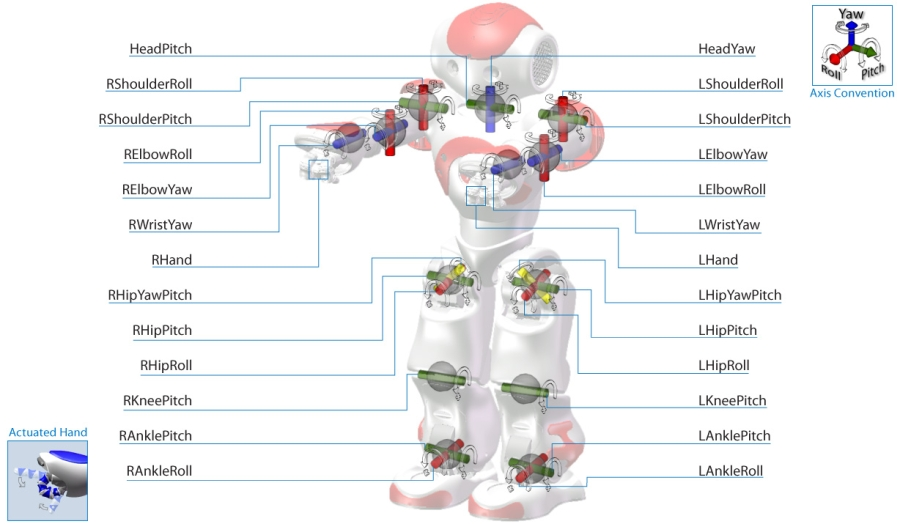
\includegraphics[width=\textwidth]{Figures/nao-robot-dof.jpeg}
\caption{Aldebaran NAO v3.3 (Academic edition) kinematic chains and joints}
\label{fig:NAO}
\end{center}
\end{figure}



\begin{figure}
\begin{tabular}{cc}
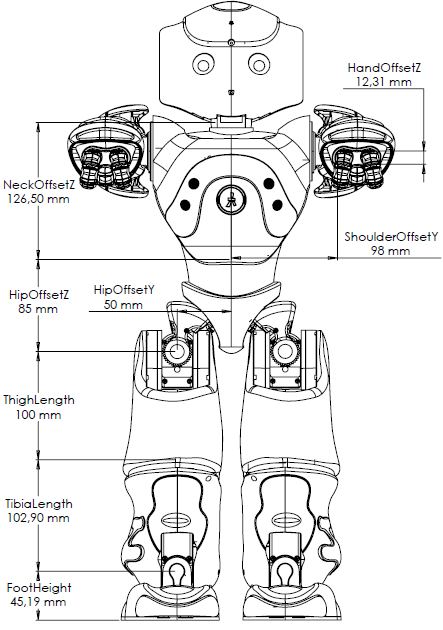
\includegraphics[height=12cm]{Figures/naolinks_1.png}
& 
\begin{tabular}{|l|l|}
\hline
{\textbf{Name}} & \textbf{Size (mm)} \\ \hline
{NeckOffsetZ} & 126.50 \\ \hline
{ShoulderOffsetY} & 98.00 \\  \hline
{ElbowOffsetY} & 15.00 \\  \hline
{UpperArmLength} & 105.00 \\  \hline
{LowerArmLength} & 55.95 \\  \hline
{ShoulderOffsetZ} & 100.00 \\  \hline
{HandOffsetX} & 57.75 \\  \hline
{HipOffsetZ} & 85.00 \\  \hline
{HipOffsetY} & 50.00 \\  \hline
{ThighLength} & 100.00 \\  \hline
{TibiaLength} & 102.90 \\  \hline
{FootHeight} & 45.19 \\  \hline
{HandOffsetZ} & 12.31 \\ \hline
\end{tabular}
\\
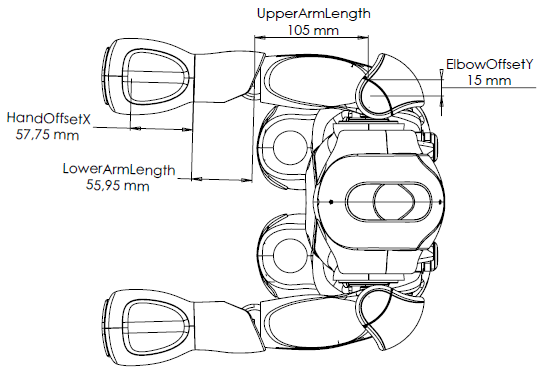
\includegraphics[height = 5cm]{Figures/naolinks_2.png}
&
\\
\end{tabular}
\caption{NAO links and their sizes}
\label{fig:NAOlinks}
\end{figure}


%\begin{figure}
%\begin{tabular}{p{9cm}l|l|}
%\multirow{14}{*}{
%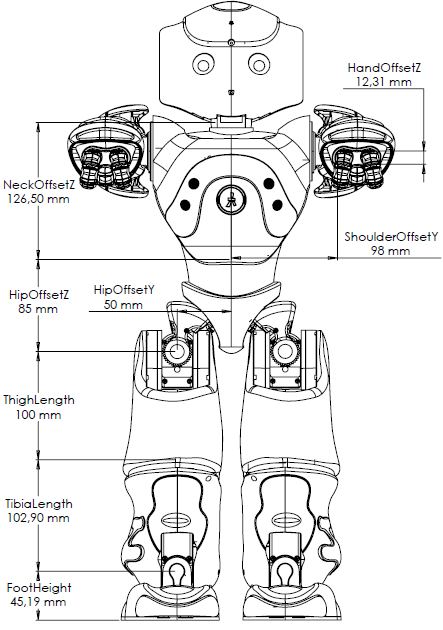
\includegraphics[height = 11cm]{Figures/naolinks_1.png}
%}
%& \multicolumn{2}{c}{} \\
%& \multicolumn{2}{c}{} \\
%& \multicolumn{2}{c}{} \\
%& \multicolumn{2}{c}{} \\
%& \multicolumn{2}{c}{} \\ \cline{2-3}
%& \multicolumn{1}{|l|}{\textbf{Name}} & \textbf{Size (mm)} \\ \cline{2-3}
%& \multicolumn{1}{|l|}{NeckOffsetZ} & 126.50 \\ \cline{2-3}
%& \multicolumn{1}{|l|}{ShoulderOffsetY} & 98.00 \\ \cline{2-3}
%& \multicolumn{1}{|l|}{ElbowOffsetY} & 15.00 \\ \cline{2-3}
%& \multicolumn{1}{|l|}{UpperArmLength} & 105.00 \\ \cline{2-3}
%& \multicolumn{1}{|l|}{LowerArmLength} & 55.95 \\ \cline{2-3}
%& \multicolumn{1}{|l|}{ShoulderOffsetZ} & 100.00 \\ \cline{2-3}
%& \multicolumn{1}{|l|}{HandOffsetX} & 57.75 \\ \cline{2-3}
% & \multicolumn{1}{|l|}{HipOffsetZ} & 85.00 \\ \cline{2-3}
%\multirow{10}{*}{
%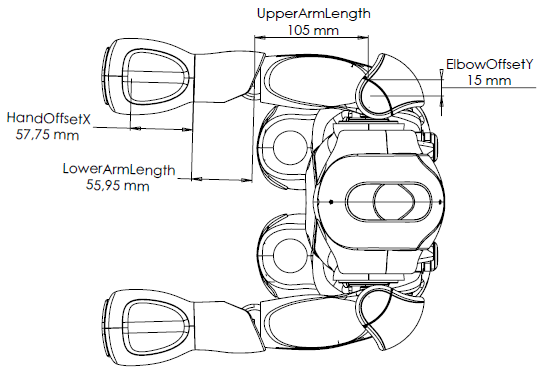
\includegraphics[height = 6cm]{Figures/naolinks_2.png}
%}& \multicolumn{1}{|l|}{HipOffsetY} & 50.00 \\ \cline{2-3}
%& \multicolumn{1}{|l|}{ThighLength} & 100.00 \\ \cline{2-3}
%& \multicolumn{1}{|l|}{TibiaLength} & 102.90 \\ \cline{2-3}
%& \multicolumn{1}{|l|}{FootHeight} & 45.19 \\ \cline{2-3}
%& \multicolumn{1}{|l|}{HandOffsetZ} & 12.31 \\\cline{2-3}
%& \multicolumn{2}{c}{} \\
%& \multicolumn{2}{c}{} \\
%& \multicolumn{2}{c}{} \\
%& \multicolumn{2}{c}{} \\
%& \multicolumn{2}{c}{} \\
%
%\end{tabular}
%\caption{NAO links sizes}
%\label{fig:NAOlinks}
%\end{figure}



\begin{figure}
\begin{tabular}{|p{5cm}|p{5cm}|p{5cm}|}
\multicolumn{3}{p{15cm}}{\centering 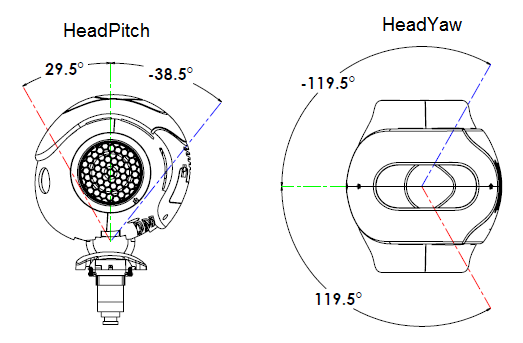
\includegraphics[height = 3.5cm]{Figures/headjoints.png}} \\ \hline
\textbf{Joint Name} & \textbf{Range in Degrees$^{\circ}$} & \textbf{Range in Radians} \\ \hline
HeadYaw & -119.5$^{\circ}$ to 119.5$^{\circ}$ & -2.0857 to 2.0857 \\ \hline
HeadPitch & -38.5$^{\circ}$ to 29.5$^{\circ}$ & -0.6720 to 0.5149 \\ \hline
\end{tabular}
\caption{NAO head joints and their operational range}
\label{fig:hjoints}
\end{figure}

\begin{figure}
\begin{tabular}{|p{5cm}|p{5cm}|p{5cm}|}
\multicolumn{3}{p{15cm}}{\centering 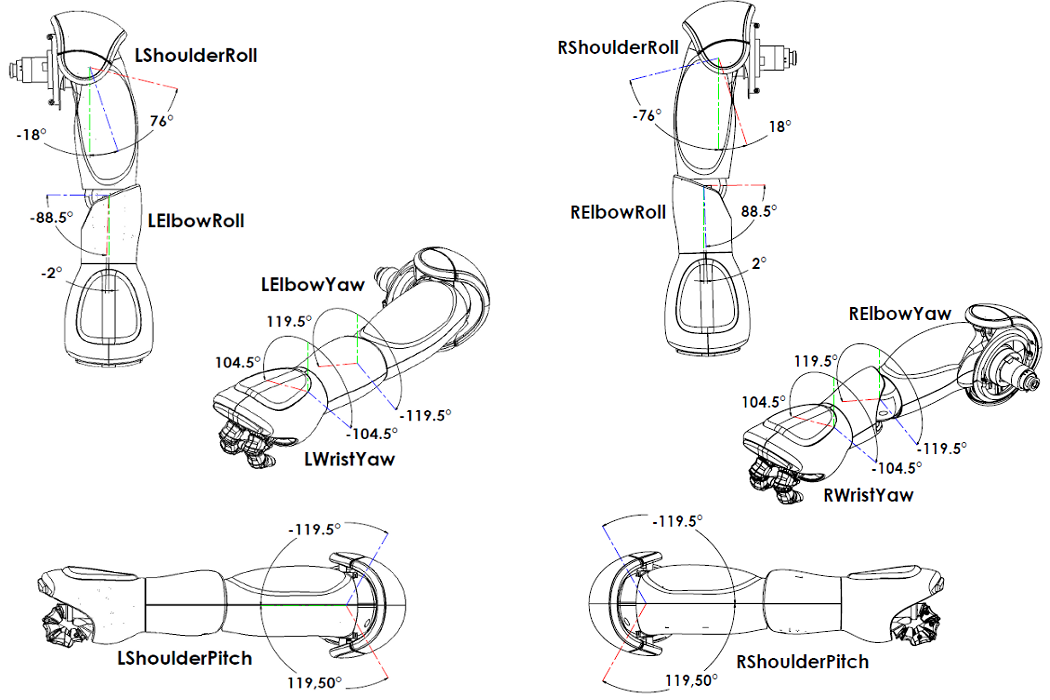
\includegraphics[height = 6.0cm]{Figures/armsjoints.png}} \\ \hline
\textbf{Joint Name} & \textbf{Range in Degrees$^{\circ}$} & \textbf{Range in Radians} \\ \hline
LShoulderPitch & -119.5$^{\circ}$ to 119.5$^{\circ}$ & -2.0857 to 2.0857 \\ \hline
LShoulderRoll & -18$^{\circ}$ to 76$^{\circ}$ & -0.3142 to 1.3265 \\ \hline
LElbowYaw & -119.5$^{\circ}$ to 119.5$^{\circ}$ & 1.5446 to 0.0349 \\ \hline
LElbowRoll & -88.5$^{\circ}$ to -2$^{\circ}$ & -0.6720 to 0.5149 \\ \hline
RShoulderPitch & -119.5$^{\circ}$ to 119.5$^{\circ}$ & -2.0857 to 2.0857 \\ \hline
RShoulderRoll & -38.5$^{\circ}$ to 29.5$^{\circ}$ & -1.3265 to 0.3142 \\ \hline
RElbowYaw & -119.5$^{\circ}$ to 119.5$^{\circ}$ & -2.0857 to 2.0857 \\ \hline
RElbowRoll & -38.5$^{\circ}$ to 29.5$^{\circ}$ & 0.0349 to 1.5446 \\ \hline
LWristYaw and RWristYaw & disabled & disabled \\ \hline
\end{tabular}
\caption{NAO arms joints and their operational range}
\label{fig:ajoints}
\end{figure}

\begin{figure}
\begin{tabular}{|p{5cm}|p{5cm}|p{5cm}|}
\multicolumn{3}{p{15cm}}{\centering 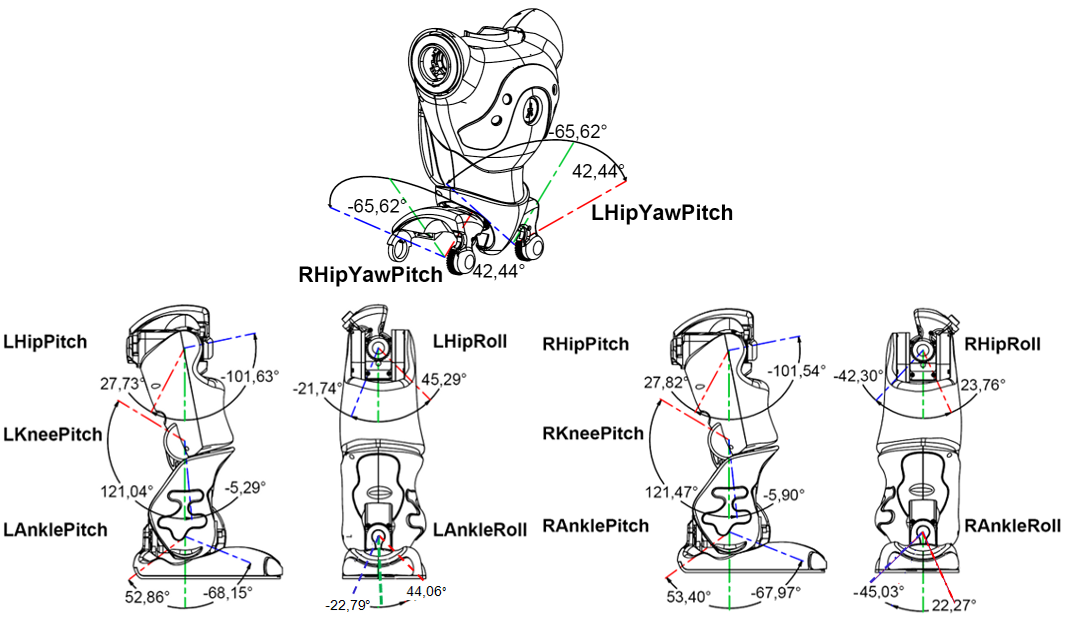
\includegraphics[width = 15cm]{Figures/legsjoints.png}} \\ \hline
\textbf{Joint Name} & \textbf{Range in Degrees$^{\circ}$} & \textbf{Range in Radians} \\ \hline
LHipYawPitch-RHipYawPitch & -65.62 to 42.44 & -1.145303 to 0.740810 \\ \hline
LHipRoll & -21.74$^{\circ}$ to 45.29$^{\circ}$ & -0.379472 to 0.790477 \\ \hline
LHipPitch & -101.63$^{\circ}$ to 27.73$^{\circ}$ & -1.773912 to 0.484090 \\ \hline
LKneePitch & -5.29$^{\circ}$ to 121.04$^{\circ}$ & -0.092346 to 2.112528 \\ \hline
LAnklePitch & -68.15$^{\circ}$ to 52.86$^{\circ}$ & -1.189516 to 0.922747 \\ \hline
LAnkleRoll & -22.79$^{\circ}$ to 44.06$^{\circ}$ & -0.397880 to 0.769001 \\ \hline
RHipRoll & -42.30$^{\circ}$ to 23.76$^{\circ}$ & -0.738321 to 0.414754 \\ \hline
RHipPitch & -101.54$^{\circ}$ to 27.82$^{\circ}$ & -1.772308 to 0.485624 \\ \hline
RKneePitch & -5.90$^{\circ}$ to 121.47$^{\circ}$ & -0.103083 to 2.120198 \\ \hline
RAnklePitch & -67.97$^{\circ}$ to 53.40$^{\circ}$ & -1.186448 to 0.932056 \\ \hline
RAnkleRoll & -45.03$^{\circ}$ to 22.27$^{\circ}$ & -0.785875 to 0.388676 \\ \hline
\end{tabular}
\caption{NAO legs joints and their operational range}
\label{fig:ljoints}
\end{figure}

\begin{table}[t!]
\caption{Masses of links/joints (frames) of the NAO robot}
\label{tab:Masses of NAO}
\begin{tabular}{|l|r|r|r|r|}
\hline
\multicolumn{5}{|c|}{\textbf{Masses for NAO v3.3 RoboCup edition}} \\ \hline
\textbf{Frame Name} & \textbf{Mass (Kg)} & \textbf{CoM$_{\text{x}}$ (mm)} & \textbf{CoM$_{\text{y}}$ (mm)} & \textbf{CoM$_{\text{z}}$ (mm)}\\ \hline
Torso & 1.03948 & -4.15 & 0.07 & 42.58 \\ \hline
HeadYaw & 0.05930 & -0.02 & 0.17 & 25.56 \\ \hline
HeadPitch & 0.52065 & 1.2 & -0.84 & 53.53 \\ \hline
RShoulderPitch & 0.06996 & -1.78 & 24.96 & 0.18 \\ \hline
RShoulderRoll & 0.12309 & 18.85 & -5.77 & 0.65 \\ \hline
RElbowYaw & 0.05971 & -25.6 & 0.01 & -0.19 \\ \hline
RElbowRoll & 0.185 & 65.36 & -0.34 & -0.02 \\ \hline
LShoulderPitch & 0.06996 & -1.78 & -24.96 & 0.18 \\ \hline
LShoulderRoll & 0.12309 & 18.85 & 5.77 & 0.65 \\ \hline
LElbowYaw & 0.05971 & -25.6 & -0.01 & -0.19 \\ \hline
LElbowRoll & 0.185 & 65.36 & 0.34 & -0.02 \\ \hline
RHipYawPitch & 0.07117 & -7.66 & 12 & 27.17 \\ \hline
RHipRoll & 0.1353 & -16.49 & -0.29 & -4.75 \\ \hline
RHipPitch & 0.39421 & 1.32 & -2.35 & -53.52 \\ \hline
RKneePitch & 0.29159 & 4.22 & -2.52 & -48.68 \\ \hline
RAnklePitch & 0.13892 & 1.42 & -0.28 & 6.38 \\ \hline
RAnkleRoll & 0.16175 & 25.4 & -3.32 & -32.41 \\ \hline
LHipYawPitch & 0.07117 & -7.66 & -12 & 27.17 \\ \hline
LHipRoll & 0.1353 & -16.49 & 0.29 & -4.75 \\ \hline
LHipPitch & 0.39421 & 1.32 & 2.35 & -53.52 \\ \hline
LKneePitch & 0.29159 & 4.22 & 2.52 & -48.68 \\ \hline
LAnklePitch & 0.13892 & 1.42 & 0.28 & 6.38 \\ \hline
LAnkleRoll & 0.16175 & 25.4 & 3.32 & -32.41 \\ \hline
\bf Total Mass & \bf 4.88083 % original: 4.879 
& \multicolumn{3}{c|}{} \\  \hline
%\multicolumn{3}{|l|}{\bf Total Mass For NAO H21} & \multicolumn{2}{|r|}{\bf 4.879 kg}\\ \hline
\end{tabular}
\end{table}

To fully specify the joints of the NAO robot, we give the length of all the links of the robot (Table~\ref{fig:NAOlinks}), the operational range in radians and degrees of the head joints (Figures~\ref{fig:hjoints}), the arm joints (Figure~\ref{fig:ajoints}), and the leg joints (Figure~\ref{fig:ljoints}), as well as the mass of each joint/link (Table~\ref{tab:Masses of NAO}). These values have been extracted from the documentation~\cite{AldebaranNaoDoc} provided by the manufacturer of the robot, Aldebaran Robotics. The center of mass for each link/joint is represented by a point in the three-dimensional space of that joint assuming a zero posture of that joint. The documentation gives mass values only for the right part of the robot; we assume that the robot is fully symmetric with respect to the sagittal plane to obtain the masses for the left part. In general, the robot is supposed to be fully symmetric, but interestingly, according to the manufacturer, some joints on the left side have a different range than the corresponding joints on the right side. Additionally, although some joints appear to be able to move within a large range, the hardware controller of the robot prohibits access to the extremes of these ranges, because of possible collisions with the NAO shell.

\section{The Kinematics Problem for NAO}
The NAO robot has a large number of DOF, therefore it can perform several complex moves. Some examples of such moves are walking, kicking a ball, standing up, etc.  Kinematics are quite useful for NAO software developers, because they can be used for planning and executing such complex movements. For example, using forward kinematics and the current joint values, one can easily find the exact position and orientation of the camera with respect to the floor the robot is standing on and therefore determine the horizon in the camera view. Likewise, using inverse kinematics, one can easily follow planned trajectories with one foot, while standing on the other, to perform dynamic kick motions. 



\subsection{The Forward Kinematics Problem for NAO}
The forward kinematics problem is to define a mapping from the joint space of the robot to the three-dimensional space with respect to any base coordinate frame.
All joints of the NAO robot are equipped with 12-bit encoders, which are updated at a frequency of 100Hz, and therefore the current joint values are readily available at any time. Despite the 21 DOF, the forward kinematics problem can be easily decomposed because three of the five kinematic chains (the head and the two arms) are completely independent and two of them (the two legs) only have one common joint. Given that in forward kinematics we do not affect the values of the joints, but only read the current state of each joint, we can assume that even the two legs chains are completely independent. Therefore, forward kinematics for NAO can been seen as five independent problems with corresponding solutions, one for each kinematic chain. Each of these solutions provides the exact point (position and orientation) in the three-dimensional space with respect to any base coordinate frame of any end effector along the corresponding kinematic joint. These solutions can be combined to obtain a solution for a bigger kinematic chain formed by any combination of the five independent chains (e.g. the kinematic chain from the right foot to the head or the kinematic chain from the left foot to the right hand). 

The importance of solving the forward kinematics problem for NAO is twofold: apart from the ability to locate the exact position and orientation of any end effector of the robot, it provides the means to calculate the center of mass of the robot for the current configuration, which is most-needed for balancing. In addition, as we shall see later, solution to the inverse kinematics problem would be intractable without solving the forward kinematics problem first.

\subsection{The Inverse Kinematics Problem for NAO}
The inverse kinematics problem is to define ways to go from the three-dimensional space of the robot to the joint space. In particular, it defines a relation between points in the three-dimensional space (position and orientation) and joint values in the joint space of a kinematic chain. For the reasons stated above, the inverse kinematics problem can be decomposed again into five independent problems. The coupling between the two legs due to the common joint is initially ignored. This is a required assumption to make the problem solvable; the obtained solutions can be combined in different ways to form a unique solution. A solution to each of these independent problems can provide the joint values which place the end effector of the corresponding kinematic chain to a specific point in the three-dimensional space of the robot torso. 

Inverse kinematics represents a much more difficult problem compared to forward kinematics for at least two reasons. First, it leads to a system of non-linear equations, which may, or may not, have an analytical solution. Second, as the number of DOF increases and the kinematic chain becomes more flexible, a point in the three-dimensional space may have more than one matching points in the joint space of the chain. This multiplicity of solutions defines a complex relation, but not a mapping, between the two spaces.

The importance of solving the inverse kinematics problem for NAO lies in the ability to follow any (predefined or dynamically-generated) trajectory in the three-dimensional space with any of the five end effectors. Inverse kinematics essentially provide the mechanism to transform such a trajectory into another trajectory in the joint space of the robot. 

The inverse kinematics problem can be solved analytically with closed-form equations or numerically with an iterative approximation method~\cite{jacobianInverse}. The analytical solution is in general faster than the fastest numerical solution and therefore is more appropriate for real-time execution. Numerical solutions are also subject to singularities, which result in a failure to obtain a solution, even if one exists. Additionally, numerical solutions are iterative; for real-time execution the number of iterations is limited and therefore they may fail to converge. For these reasons, we aim to find an analytical solution to the inverse kinematics problem for the NAO robot. It is well-known that inverse kinematics can be obtained analytically, if the chain has five or less DOF. If the chain has six DOF, an analytical solution can be obtained, only if three sequential joints have intersecting axes. Three of the kinematics chains of the NAO robot have less than five DOF. The legs have six DOF, however the meet the condition given above because the three hip joints have intersecting axes. Therefore, it is possible to obtain a fully analytical solution for the inverse kinematics of the NAO. 


\section{Related Work}

The problem of forward and inverse kinematics for the NAO robot is a familiar problem to all the teams participating in RoboCup SPL. The solution to forward kinematics is quite straightforward and most teams have implemented their own code for forward kinematics computations. There are only a few known solutions for the problem of inverse kinematics. We review existing related work in the next few sections. 

\subsection{Aldebaran Robotics}

%\subsubsection*{Aldebaran Forward Kinematics Solution}
Aldebaran Robotics provides a forward kinematics mechanism integrated within the proprietary NaoQi middleware for the NAO robot. However, this mechanism does not accept any input and provides a solution only for the current joint configuration of the robot. As a result, it is impossible to run Aldebaran's forward kinematics for a specific set of joint values, for example the joint values recorded when a specific picture was acquired from the camera. The ability to provide any set of joints is important, not only for finding the position of the camera in the three-dimensional at specific times, but also for verifying candidate solutions returned by inverse kinematics. On the other hand, Aldebaran provides the DH parameters for all the joints of the NAO robot and that was very useful.

%\subsubsection*{Aldebaran Inverse Kinematics Solution}
Aldebaran Robotics provides an inverse kinematics mechanism integrated within the proprietary NaoQi middleware for the NAO robot. These functions in the API of the robot can move the end effector of a kinematic chain to a given point in the three-dimensional space. The method used to provide the solution is based on the Jacobian iterative approximation method. Furthermore, the omni-directional walk engine provided by Aldebaran Robotics uses this approach to follow planned foot trajectories. Although the resulting solutions are in most cases accurate, the method can easily fall into singularities; if that happens, the robot gets stuck in a specific configuration. Singularities present a serious problem with possible catastrophic consequences for the robot. 

\subsection{B-Human Inverse Kinematics Solution}
B-Human is the RoboCup SPL team of the University of Bremen in Germany. Each year they publish a code release, which includes the full code they used in the last RoboCup and a documentation for this code. In their recent code release~\cite{bhuman} they include an inverse kinematics solution for the legs of NAO, albeit with under certain simplification assumptions and approximations. The solution provided always makes the foot parallel to the plane defined by the $z$-axis and the $x$-axis of the torso. If the target point violates this assumption, the solution will reach the target position, but will ignore the target orientation, and therefore it will only be an approximate solution. 

\subsection{QIAU Inverse Kinematics Solution}
MRL is the RoboCup SPL team of the Qazvin Islamic Azad University (QIAU) in Tehran, Iran. They have published~\cite{iran} an analytical solution for the problem of inverse kinematics for the legs. We have tried to implement their solution, but unfortunately we were not able to reproduce their results.




% ------------------------------------------------------------------------

%%% Local Variables:
%%% mode: latex
%%% TeX-master: "../thesis"
%%% End:
